\documentclass[11pt]{article}

% ---------------------------------------------------------------------------
% Preamble — arXiv-style single-column preprint
% ---------------------------------------------------------------------------
\usepackage[a4paper, margin=1.1in]{geometry}
\usepackage[utf8]{inputenc}
\usepackage[T1]{fontenc}
\usepackage{lmodern}
\usepackage{microtype}
\usepackage{amsmath, amssymb}
\usepackage{booktabs}
\usepackage{graphicx}
\usepackage{caption}
\usepackage{subcaption}
\usepackage{xcolor}
\usepackage{tikz}
\usetikzlibrary{positioning, arrows.meta, calc}
\usepackage{url}
\urlstyle{tt}
\usepackage[round]{natbib}
\usepackage[colorlinks=true, linkcolor=blue!60!black, citecolor=blue!60!black, urlcolor=blue!60!black]{hyperref}

% Give TeX room to avoid overfull lines around long typewriter strings
\emergencystretch=1.5em

% Placeholder machinery: every number or figure that does not exist yet is
% marked in red so nothing unfinished can hide in the final read-through.
\newcommand{\todo}[1]{\textcolor{red}{[TODO: #1]}}
\newcommand{\resultnum}[1]{\textcolor{red}{$\langle$#1$\rangle$}}

% Cell shorthands, used everywhere for consistency
\newcommand{\cellhm}{\textsc{hum-mono}}
\newcommand{\cellhd}{\textsc{hum-dia}}
\newcommand{\cellad}{\textsc{ai-dia}}
\newcommand{\cellam}{\textsc{ai-mono}}
\newcommand{\cellrt}{\textsc{ai-reason}}

\title{Monologue or Dialogue?\\
\large Measuring Conversational Structure in the Reasoning Traces\\ of Large Language Models}

\author{%
  Oskar Engl\\
  Johannes Kepler University Linz, Austria\\
  \texttt{oskar.engl@ik.me}%
}

\date{\today, working draft}

\begin{document}
\maketitle

% ---------------------------------------------------------------------------
\begin{abstract}
Reasoning models such as DeepSeek-R1 produce a long ``thinking'' trace before
they answer. Such a trace can read as a single mind reasoning step by step, or
as several voices trading proposals and objections. We ask which of these
descriptions the text better fits when the question is put to measurement.
There is no established ground truth for the voice structure of a reasoning
trace, so we assemble a $2{\times}2$ grid of corpora whose structure \emph{is}
known (human and AI, monologue and dialogue) and let a detection method judge
the reasoning traces only after it has performed satisfactory \todo{would be nice if 
you could make this "satisfactors" a link to where we explain the criteria 
exactly} on distinguishing monologue from dialogue on the four
known corpora. Three methods are tested, each reading a different textual
signal: a document-level single- versus multi-author classifier
\citep{nath2019style}, a sentence-level detector of where the writing style
switches \citep{schmidt2025sspc}, and dialogue-act tagging that measures
conversational structure through adjacency pairs \citep{duran2022cams,
schegloff1973opening}. All analysis decisions were fixed and placed under
version control before any statistic was computed on the reasoning traces.
\todo{One sentence stating the verdict pattern: which methods passed the
validity check, and whether R1 traces read as monologue, dialogue, or mixed.}
\end{abstract}

% ---------------------------------------------------------------------------
\section{Introduction}
\label{sec:intro}

Reasoning-oriented training has become standard in frontier language models:
given a problem, a model such as DeepSeek-R1 \citep{deepseek2025r1} first
generates an extended stretch of intermediate tokens \todo{please cite the 
paper Position: Stop Anthropomorphizing Intermediate Tokens as Reasoning/Thinking 
Traces! here, wherever you think exactly it fits best. i think this is great to 
mention in the context of the definition of intermediate tokens.}, a \emph{reasoning
trace}, and only then commits to an answer. These traces have a curious
property: Each is produced by a single model in one generation pass, yet a
trace often contains questions and the answers to them, objections and
concessions, and abrupt reversals (``Wait, that's not right''). In text
written by people, such features can mark a genuine exchange between
participants, though they can equally mark a single vivid inner voice. This
raises a question that is easy to state and less easy to settle: \emph{does a
reasoning trace have the textual structure of a monologue or of a dialogue?}

[oskars bookmark] 

\citet{kim2026societies} argue,
drawing on both interpretability analysis and automatic labeling of the
traces, that reasoning-trained models improve in part because they simulate a
``society of thought'': distinct internal perspectives that propose,
criticize, and reconcile. Cognitive science offers older versions of the same
idea: \citet{mercier2017enigma} hold that human reasoning is at root
argumentative and social, and \citet{minsky1986society} modeled the mind as
many interacting agents. Against this background, the monologue-or-dialogue
question becomes a test one can actually run: if reasoning traces carry the
measurable structure of dialogue, that is evidence consistent with these
accounts; if they do not, the impression of an inner conversation may owe
more to the reader than to the text.

Our premise is that voice structure leaves marks in the writing itself. The
society-of-thought account describes the internal perspectives as differing
in role and character \citep{kim2026societies}; if distinct perspectives take
turns producing the text, they should also differ in how they write, in the
small, largely involuntary habits (function-word use, sentence rhythm,
dialogue-act moves) that authorship analysis uses to tell writers apart. We
therefore treat the question operationally: a monologue should read as one
author, a dialogue as several, and we ask which of these the reasoning traces
resemble. This is not the setting these methods were built for: their
``authors'' are ordinarily different people, not perspectives within one
model. Section~\ref{sec:related} returns to what that borrowing does and
does not license.

No corpus of reasoning traces comes labeled with its true voice structure,
which is what makes the question hard to settle directly. We address this with
the grid in Figure~\ref{fig:design}. We assemble four corpora whose structure
is known: human monologue (think-aloud protocols), human dialogue (group
deliberation), AI monologue (one model solving a puzzle alone), and AI
dialogue (four instances of one model, each given a different role,
debating), alongside the reasoning traces themselves. A method may report on
the traces only after it has correctly separated monologue from dialogue on
all four known corpora; a method that fails this check is reported as failing
and set aside.

The three methods read different signals. Two come from authorship analysis
and the PAN style-change task \citep{zangerle2025pan}: one classifies a whole
document as single- or multi-author from its function-word profile
\citep{nath2019style}, while the other works sentence by sentence, estimating
at each point whether the writing style has switched \citep{schmidt2025sspc}.
The third comes from conversation analysis: it labels each utterance with its
dialogue act and checks for adjacency pairs, a question followed by an
answer, a proposal by its acceptance or refusal, which
\citet{schegloff1973opening} describe as a basic unit of conversational
organization. The first two share this lineage but differ in mechanism; the
third is unrelated to either. Because they read the text in different ways,
agreement among them carries more weight than any one method alone.

Two further choices shape the design. First, we hold the task fixed: the AI
monologue, AI dialogue, and reasoning-trace corpora all solve the same
puzzle, Game of 24 \citep{yao2023tree}. The methods examine style and
structure rather than subject matter, so the risk of one keying on topic is
small to begin with; holding the task constant removes it and keeps as many
variables fixed as possible. Second, pre-registration: every analysis rule,
threshold, and figure was fixed and version-controlled before any statistic
was computed on the reasoning traces (Section~\ref{sec:prereg}).

\paragraph{Contributions.}
We (i) frame the monologue-or-dialogue question about reasoning traces as a
measurable comparison against corpora of known voice structure; (ii) evaluate
three established detection methods on matched human and AI, monologue and
dialogue corpora, admitting each to the reasoning traces only after it passes
a validity check on the known corpora; and (iii) \todo{report the verdict on
DeepSeek-R1 traces}.

% ---------------------------------------------------------------------------
\begin{figure}[t]
\centering
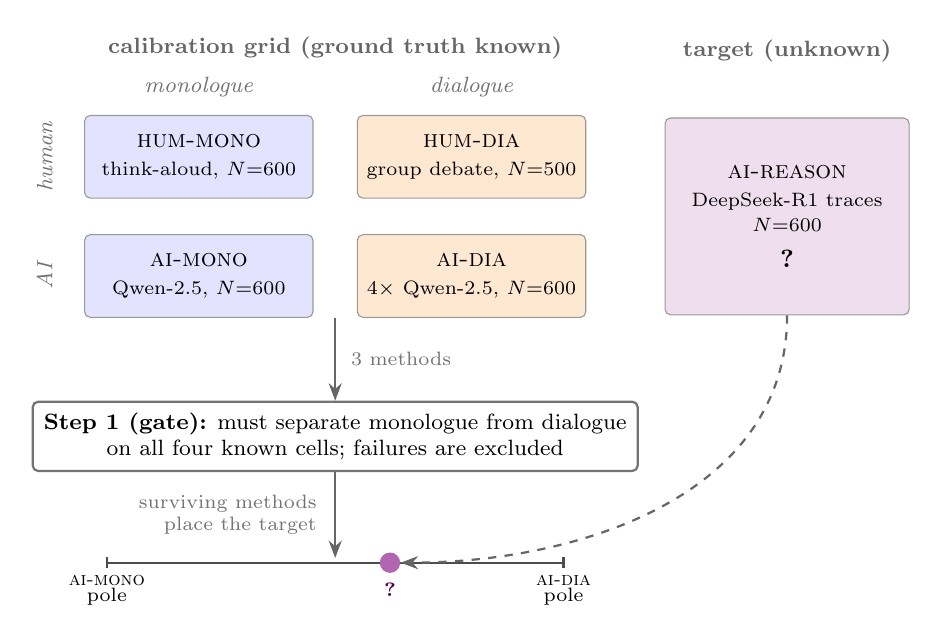
\begin{tikzpicture}[
  font=\small,
  cellbox/.style={draw=black!40, rounded corners=2pt, minimum width=2.9cm,
    minimum height=1.05cm, align=center, inner sep=3pt},
  mono/.style={cellbox, fill=blue!11},
  dia/.style={cellbox, fill=orange!18},
  tgt/.style={cellbox, fill=violet!13, minimum height=2.5cm, minimum width=3.1cm},
  meth/.style={draw=black!40, rounded corners=2pt, fill=black!4,
    minimum width=3.55cm, minimum height=0.85cm, align=center, font=\footnotesize},
  gate/.style={draw=black!55, thick, rounded corners=2pt, fill=white,
    align=center, font=\footnotesize, inner sep=4pt},
  lbl/.style={font=\footnotesize\itshape, text=black!55},
  arr/.style={-{Stealth[length=2.2mm]}, black!60, thick}
]
% --- calibration grid ---
\node[mono] (hm) {\cellhm\\[-1pt]\scriptsize think-aloud, $N{=}600$};
\node[dia, right=0.55cm of hm] (hd) {\cellhd\\[-1pt]\scriptsize group debate, $N{=}500$};
\node[mono, below=0.45cm of hm] (am) {\cellam\\[-1pt]\scriptsize Qwen-2.5, $N{=}600$};
\node[dia, below=0.45cm of hd] (ad) {\cellad\\[-1pt]\scriptsize $4\times$ Qwen-2.5, $N{=}600$};
\node[lbl, above=0.10cm of hm] {monologue};
\node[lbl, above=0.10cm of hd] {dialogue};
\node[lbl, rotate=90, anchor=south] at ($(hm.west)+(-0.28,0)$) {human};
\node[lbl, rotate=90, anchor=south] at ($(am.west)+(-0.28,0)$) {AI};
\node[font=\footnotesize\bfseries, text=black!60] at ($(hm.north)!0.5!(hd.north)+(0,0.85)$)
  {calibration grid (ground truth known)};
% --- target ---
\node[tgt] (rt) at ($(hd.east)!0.5!(ad.east)+(2.55,0)$)
  {\cellrt\\[-1pt]\scriptsize DeepSeek-R1 traces\\[-2pt]\scriptsize $N{=}600$\\[2pt]\textbf{?}};
\node[font=\footnotesize\bfseries, text=black!60] at ($(rt.north)+(0,0.85)$) {target (unknown)};
% --- gate ---
\node[gate, below=1.05cm of $(am.south)!0.5!(ad.south)$] (g)
  {\textbf{Step 1 (gate):} must separate monologue from dialogue\\on all four known cells; failures are excluded};
\draw[arr] ($(am.south)!0.5!(ad.south)$) -- (g.north)
  node[midway, right=2pt, font=\scriptsize, text=black!55] {3 methods};
% --- placement axis ---
\coordinate (axL) at ($(g.south)+(-2.9,-1.15)$);
\coordinate (axR) at ($(g.south)+(2.9,-1.15)$);
\draw[black!70, thick] (axL) -- (axR);
\foreach \x in {axL, axR} \draw[black!70, thick] (\x)+(0,0.07) -- ($(\x)+(0,-0.07)$);
\node[font=\scriptsize, below=1pt of axL, align=center] {\cellam\\[-2pt]pole};
\node[font=\scriptsize, below=1pt of axR, align=center] {\cellad\\[-2pt]pole};
\node[circle, fill=violet!60, inner sep=2.6pt, label={[font=\scriptsize\bfseries, text=violet!60!black]below:?}]
  (q) at ($(axL)!0.62!(axR)$) {};
\draw[arr] (g.south) -- ($(axL)!0.5!(axR)+(0,0.06)$)
  node[midway, left=3pt, font=\scriptsize, text=black!55, align=right]
  {surviving methods\\place the target};
\draw[arr, dashed] (rt.south) to[out=-90, in=0, looseness=1.0] (q.east);
\end{tikzpicture}
\caption{Study design. Four corpora with known voice structure (left) gate
the three detection methods: a method may report on the target only after it
separates monologue from dialogue on all four. Methods that pass then place
the target on a monologue--dialogue axis anchored by the two same-task AI
cells; the human cells are used only for validation, not for placement.}
\label{fig:design}
\end{figure}

% ---------------------------------------------------------------------------
\section{Related Work}
\label{sec:related}

\paragraph{Multi-author and style-change detection.}
Stylometry rests on the observation that unconscious habits, such as
function-word frequencies and character n-grams, are stable within an author and vary between
authors \citep{stamatatos2008survey}. The PAN shared-task series has posed
style-change detection since 2016: given a document, decide whether one or
several authors wrote it, and where the switches occur
\citep{zangerle2019pan, zangerle2025pan}. Our Method~1 is the threshold-based
clustering approach of \citet{nath2019style} from the PAN 2019 edition; our
Method~2 is a sequential sentence-pair classifier submitted to the PAN 2025
edition \citep{schmidt2025sspc}, built on content-independent style
embeddings \citep{patel2025styledistance}. Stylometric analysis of
multi-authored documents more broadly is surveyed by
\citet{zamir2024stylometry}. We repurpose this machinery for a question it was
not designed for. In the original task the several authors are different
people; here they would be perspectives within a single model's output. The
justification is the premise stated in Section~\ref{sec:intro}: the
society-of-thought account attributes distinct roles and characters to these
perspectives \citep{kim2026societies}, and writers with distinct characters
tend to leave distinct stylistic marks. Whether that assumption holds for one
model's text is part of what the known-structure corpora are there to test.

\paragraph{Dialogue structure and conversation analysis.}
In conversation analysis, a dialogue is not just alternating text but a system
of paired actions. \citet{schegloff1973opening} describe the \emph{adjacency
pair}: two turns by different speakers in which the first makes the second
relevant: a question makes an answer due, an offer makes an acceptance or a
refusal due. This pairing is a basic way conversation is organized, and its
two parts normally sit next to each other. Dialogue-act schemas make the
pattern measurable by labeling each utterance with its function; we use the
Conversation Analysis Modelling Schema \citep[CAMS;][]{duran2022cams}, which
pairs a dialogue-act layer with adjacency-pair types. Adjacency-pair
completion is the property that matters here, because a lone writer has little
reason to produce it: a monologue may pose rhetorical questions, but it rarely
answers them in the very next utterance the way a conversation does. Whether
solitary human thought is itself monological is contested: in the Vygotskian
tradition, inner speech is internalized dialogue and can keep the give-and-take
of the conversations it grew from \citep{fernyhough2004, aldersonday2015}. Our
design need not settle this: here ``monologue'' is defined by production, one
speaker alone, and whatever dialogic residue a lone speaker's talk carries is
what the known-structure corpora teach the methods to accept as a single
voice.

\paragraph{Reasoning traces and their interpretation.}
Chain-of-thought prompting showed that intermediate text improves model
problem-solving \citep{wei2022cot}; reasoning-oriented training internalized
the behavior \citep{deepseek2025r1}. What the resulting traces \emph{are} is
contested. \citet{kim2026societies} report that reasoning models engage
diverse, sometimes conflicting internal perspectives, and that this shows up
in the traces as conversational behavior: question-answer sequences, shifts
in perspective, and the reconciliation of competing views. They reach this
through several routes, including mechanistic interpretability and LLM-based
labeling of the traces into distinct personas. Our study is narrower and
complementary: we take a small set of established text-level methods, each
with an explicit validity check on corpora of known structure, and ask only
whether the traces sit closer to monologue or to dialogue. On the human side,
think-aloud protocol analysis \citep{ericsson1984protocol} treats verbalized
solitary reasoning as data; \citet{wurgaft2025thinkaloud} scale the method
with automated transcription and coding, producing the Game-of-24 think-aloud
corpus we use as our human-monologue cell. For human dialogue we draw on
DeliData \citep{karadzhov2023delidata}, 500 group deliberations on the Wason
card-selection task \citep{wason1968reasoning}.

% ---------------------------------------------------------------------------
\section{Study Design and Data}
\label{sec:design}

\subsection{The calibration grid}
\label{sec:grid}

The design is a $2{\times}2$ grid plus one target cell
(Figure~\ref{fig:design}, Table~\ref{tab:cells}). The grid cells vary
producer (human vs.\ AI) and structure (monologue vs.\ dialogue), and for
each the true structure is known, either by construction or from the source
the corpus was collected from. The fifth cell, native DeepSeek-R1 reasoning
traces, is the object of study.

\begin{table}[t]
\centering
\caption{The five corpora (``cells''). The four calibration cells have known
voice structure; the target does not. $N$ = documents per cell.}
\label{tab:cells}
\footnotesize
\begin{tabular}{@{}llllr@{}}
\toprule
Cell & Structure & Producer & Task & $N$ \\
\midrule
\cellhm{} & monologue & humans thinking aloud \citep{wurgaft2025thinkaloud} & Game of 24 & 600 \\
\cellhd{} & dialogue & human groups, DeliData \citep{karadzhov2023delidata} & Wason selection & 500 \\
\cellam{} & monologue & Qwen-2.5-7B, task-only prompt & Game of 24 & 600 \\
\cellad{} & dialogue & $4\times$ Qwen-2.5-7B, stateless debate & Game of 24 & 600 \\
\midrule
\cellrt{} & \textbf{unknown} & DeepSeek-R1, native thinking mode & Game of 24 & 600 \\
\bottomrule
\end{tabular}
\end{table}

$N=600$ was chosen as a practical balance between statistical power and
generation/annotation cost for the four cells we control (\cellhm{},
\cellam{}, \cellad{}, \cellrt{}); \cellhd{} is fixed at $N=500$ by the size of
the DeliData corpus itself, since no larger matched human-dialogue dataset
exists. We do not treat the resulting imbalance as a design choice worth
defending on statistical grounds. The pre-registered gates are constructed to
be insensitive to unequal cell sizes (balanced accuracy, Cliff's $\delta$,
per-cell reliability sample sizes).

The grid works as a gate: a method may report on the target only after it
correctly separates monologue from dialogue on all four known cells
(Section~\ref{sec:methods}). A method that cannot tell the four voices apart
in a genuine four-way debate is in no position to rule them out in a reasoning
trace; a method that reports several voices in a lone person's think-aloud
protocol is in no position to affirm them there.

\subsection{Task control}
\label{sec:task}

A detection method can respond to what a text is about, not only to how many
voices produced it, and the domain of a task can shape a text's structure. To
keep such influences from being mistaken for voice structure, we hold the task
fixed wherever possible: \cellam{}, \cellad{}, and \cellrt{} all solve Game of
24 \citep{yao2023tree}: combine four given numbers arithmetically to reach
24, and \cellhm{} uses the same puzzle, so a method reading human monologue as
a single voice cannot be doing so merely in reaction to the puzzle. \cellhd{}
is the exception: DeliData is built around the Wason card-selection task, and
no Game-of-24 group-deliberation corpus exists. We chose the Wason task because
it is likewise a compact logic puzzle, the closest human group-deliberation
data we could find to Game of 24. Its role is limited, to confirm that a
method detects human dialogue at all, so we do not use it as a placement
anchor (Section~\ref{sec:placement}). The comparison that carries the placement
is the same-task AI set: \cellam{} vs.\ \cellad{} vs.\ \cellrt{}.

\subsection{Generated cells}
\label{sec:generation}

\textbf{AI monologue (\cellam{}).} One call per puzzle to an
instruction-tuned model (\path{qwen/qwen-2.5-7b-instruct}), with a minimal
prompt that states the puzzle and its rules and asks for a solution, imposing
no further structure on the response (Appendix~\ref{app:generation}).

\textbf{AI reasoning traces (\cellrt{}).} One call per puzzle to DeepSeek-R1
(\path{deepseek/deepseek-r1}) in its native thinking mode, using the same
minimal prompt as \cellam{}. The document is the model's reasoning trace,
taken from the thinking channel of the response.

\textbf{AI dialogue (\cellad{}).} This cell needed the most care, because the
multiplicity has to come from separate model calls rather than from a single
call asked to write several parts. Four instances of the same model
(\path{qwen/qwen-2.5-7b-instruct}, as in \cellam{}) take turns writing the
debate, one API call per turn. The instances are stateless and share only the
running transcript: at each turn the current speaker sees the debate so
far, the turns the other participants have written, and nothing else. Each
is given a fixed role (creative problem solver, critical analyst, mathematical
validator, alternative seeker) and a name, a letter A--D, so the participants
can address one another. Turn order is drawn at random. A debate ends once all
four participants have spoken and the exchange has either signalled a
conclusion or begun to repeat itself, or at a hard cap of 40 turns;
Appendix~\ref{app:generation} gives the exact stopping rule. Two features of
this setup are worth noting. We use four instances of one model rather than
four different models, because the reasoning traces we study also come from a
single model: if a method cannot find multiple voices in a same-model debate,
that reflects the method's sensitivity, which the gate records. And no single
call is ever asked to produce the whole four-person exchange, because a single
call performing many voices is the very thing we are trying to detect in the
reasoning traces and so cannot also serve as a positive control. The two
anchors share one base model (Qwen-2.5-7B), while the target is a different
model (DeepSeek-R1); Section~\ref{sec:limitations} discusses the implications.

\subsection{Acknowledged confounds}
\label{sec:confounds}

\begin{figure}[t]
\centering
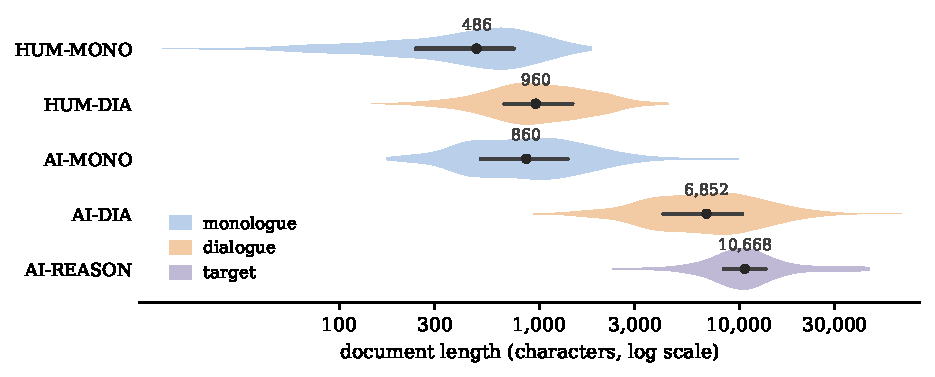
\includegraphics[width=0.92\textwidth]{figures/fig_lengths.pdf}
\caption{Document length per cell (log scale; violins with median dot,
interquartile bar, and annotated median). Length differences follow from the
design: dialogue produces more text than monologue, and the reasoning traces
are longer than both AI anchors. Each cell shows its 600-document analysis
sample (\cellhd{}: 500).}
\label{fig:lengths}
\end{figure}

Several properties of the corpora could influence a method's output alongside
voice structure; we state them here and return to them in
Section~\ref{sec:limitations}. First, in the human pair, \cellhm{} and
\cellhd{} differ in task as well as structure (Game of 24 vs.\ Wason), so a
method's success in separating them could partly reflect task; this is why the
human pair only validates and the AI set carries the placement. Second, the
four debate roles in \cellad{} may add stylistic variation beyond
multiplicity itself, though we take role differentiation to be part of what
multiplicity means here, following the society-of-thought account
\citep{kim2026societies}, in which distinct perspectives are distinct roles;
a positive style-method result on \cellad{} should be read as an upper bound
on the role-free component. Third, \cellhm{} is transcribed speech while every
AI cell is written text, so human--AI comparisons mix producer with register.
Fourth, document lengths span two orders of magnitude across cells
(Figure~\ref{fig:lengths}), and the reasoning traces are longer than either
anchor; Section~\ref{sec:method2} shows where this matters and how we handle
it.

% ---------------------------------------------------------------------------
\section{Methods}
\label{sec:methods}

Each of the three methods follows the same procedure. First we calibrate it:
run it on the four known cells and test it against a validity gate (defined
per method below). A method that passes is then applied, unchanged, to the
reasoning traces; a method that fails is reported and set aside. Reading a
surviving method's result means placing the reasoning traces on a
monologue--dialogue axis anchored by the two AI cells, \cellam{} and
\cellad{} (Section~\ref{sec:placement}). The three methods work on different
signals: a function-word frequency clustering, a pretrained neural style
encoder (with NLTK Punkt sentence splitting; \citealp{bird2009nltk}), and an
LLM dialogue-act tagger, and are run independently of one another.

\subsection{Method 1: Document-level style-change detection}
\label{sec:method1}

\citet{nath2019style} estimates how many authors wrote a document by
clustering its paragraph-sized windows on their function-word profiles. The 50
most frequent tokens of the document define a small feature space, and each
window is described by how often those tokens occur within it; windows are
then compared by Matusita distance and grouped by threshold-based clustering
(TBC), with the number of resulting clusters taken as the author count. We use
the author's own implementation in the configuration it reports as best, and
make two corrections so that our run matches the method as the paper describes
it. The shipped script defaults to a different distance measure, which we set
back to the Matusita distance the paper evaluates. And a filtering step in the
code discards paragraphs shorter than 200 characters, whereas the paper
specifies merging them into the preceding window; we restore the merging
behavior, since our debate turns are often short and discarding them would
remove exactly the turns that carry the dialogue structure.

Windowing follows the shape of each cell. In PAN's forum data a paragraph is
one person's post, so for our turn-structured cells (\cellad{}, \cellhd{}) we
treat one turn as one paragraph. The continuous-prose cells (\cellhm{},
\cellam{}, \cellrt{}) have no such natural unit; for these we rely on the
implementation's own handling, which splits a document on its blank lines and,
where a document has none, as with transcribed speech in \cellhm{}, falls
back to grouping ten sentences per window and splitting overlong paragraphs at
five sentences.

\textbf{Output.} Each document receives a predicted author count, which we
reduce to a binary call (multi-author if the count exceeds one).
\emph{Gate: balanced accuracy across the four calibration cells must
significantly exceed the trivial baseline.} We use balanced accuracy---the
mean of single-author recall (cells \cellhm{}, \cellam{}) and multi-author
recall (cells \cellhd{}, \cellad{})---rather than pooled accuracy, because the
cells are class-imbalanced (${\approx}1{,}200$ single- vs.\ ${\approx}1{,}100$
multi-author documents): a degenerate detector that labels every document
single-author scores ${\approx}0.52$ pooled and could clear a binomial test
against 0.5 on sample size alone, whereas it scores exactly 0.50 balanced, so
passing requires genuinely detecting multi-voice text. Significance is assessed
by a label-permutation null (10{,}000 shuffles of the true labels; one-sided
$p<.05$), which centres at 0.50 irrespective of the imbalance; we report
per-class recalls, the per-cell breakdown, a confusion matrix, and a bootstrap
95\% CI on balanced accuracy. We do not import the original paper's 0.85
accuracy as a threshold: that was its best score in its own domain (long
StackExchange threads), and our data are short puzzle transcripts, so we ask
only that the method distinguish single- from multi-author text better than the
trivial baseline.

\subsection{Method 2: Sentence-level style-change detection}
\label{sec:method2}

The sequential sentence-pair classifier of \citet{schmidt2025sspc} encodes
each sentence with a content-independent style embedding
\citep{patel2025styledistance}, contextualizes the sequence with a BiLSTM,
and emits, for every adjacent sentence pair, the probability that the two
sentences were written by different authors. We run the shipped pretrained
checkpoint as is, which amounts to out-of-domain inference, with no
fine-tuning on our data, and read out the raw per-pair probabilities before
any thresholding.
The per-document raw score is the mean of these probabilities: a scalar in
$[0,1]$, higher meaning more style switching.

\textbf{Length.} The reasoning traces are much longer than either anchor
(median 10{,}668 characters vs.\ 6{,}852 for \cellad{} and 860 for \cellam{};
Figure~\ref{fig:lengths}), and length affects the raw mean directly. A longer
document is divided into more sentence pairs, so if a document carries some
roughly fixed number of genuine style switches, spreading them over more pairs
lowers the mean; a raw sum has the opposite problem, growing with length even
at a constant rate of chance switches. Rather than choose between the two, we
model the length relationship on the calibration data. For each anchor
separately, using only that anchor's documents, we fit a curve of switch
probability against document length, choosing among linear, semi-log, and
log-log forms by AIC \citep{akaike1974}, so that the two anchors need not share
a functional form. Each document then receives two residual distances:
$d_{\mathrm{dia}}$, its deviation from the \cellad{} curve at its own length,
and $d_{\mathrm{mono}}$, its deviation from the \cellam{} curve. The
per-document score, which we call the \emph{lean}, is
$\ell = |d_{\mathrm{mono}}| - |d_{\mathrm{dia}}|$; a positive value means the
document sits closer to the dialogue curve. Because the reasoning traces run
past both anchors' observed length ranges, we show the extrapolation directly
(Figure~\ref{fig:m2-extrapolation}).

\textbf{Gate.} Mean lean for the dialogue cells (\cellhd{}, \cellad{}) must
exceed that for the monologue cells (\cellhm{}, \cellam{}), with Cliff's
$\delta \geq 0.33$ \citep{cliff1993dominance} between the two groups, a
direction check with a medium-effect-size floor, so that a technically
correct but negligible separation does not count as validation.

\subsection{Method 3: Dialogue-act structure}
\label{sec:method3}

Every document is segmented into utterances, and each utterance is labeled
with one of the 27 CAMS dialogue-act tags \citep{duran2022cams}, plus
\texttt{none}, by an LLM tagger with a fixed prompt at temperature~0
(Appendix~\ref{app:tagging}). For example, ``Wait, does $6\times4$ actually
give 24?'' is tagged \texttt{checkQuestion}, and a following ``Yes, that
works'' is tagged \texttt{confirm}. We use only the dialogue-act layer of
CAMS: its formal adjacency-pair annotation layer requires speaker-turn
structure that three of our five cells do not have. From the tag sequences we
compute three signals of increasing stringency, identically for every cell.

\textbf{(a) Tag distribution.} For each cell, the normalized frequency of each
of the 28 labels across all of its utterances, giving a 28-dimensional profile.
Does the reasoning traces' mix of conversational functions resemble the
monologue cells or the dialogue cells?

\textbf{(b) Tag transitions.} The $28{\times}28$ matrix of counts of one tag
immediately following another. Because a transition must stay within a single
document (the last tag of one document does not precede the first tag of the
next), these counts are formed per document and then summed within each cell:
which conversational move tends to follow which?

\textbf{(c) Adjacency-pair completion (primary signal).} Signals (a) and (b)
are profiles; a monologue that merely \emph{contains} many questions could
score dialogue-like on them. Signal (c) tests what adjacency-pair theory
identifies as the mark of conversation: when a first pair-part (FPP)
occurs (a question, request, suggestion, offer), is it met by a valid second
pair-part (SPP) in the \emph{very next} utterance? The mapping from each FPP
tag to its valid responses (Table~\ref{tab:fpp-spp}) is derived from CAMS's
category structure and was fixed before any data was seen. The per-document
metric is the \emph{completion rate}: of all adjacent tag pairs whose first
member is an FPP, the fraction whose second member is a valid SPP. A document
that contains no FPP has a completion rate of 0 (it initiates no pairs to
complete); we also report, per cell, the share of such documents, since a
monologue cell is expected to contain many. We require immediate
adjacency: the SPP in the very next utterance, with no inserted material,
which CAMS allows but which needs speaker structure to detect. This keeps the
measure conservative: by ignoring completions separated by an insertion, it
can only understate how often pairs are completed, so any dialogue-ward
difference it produces is not an artifact of a lenient criterion.%
\todo{FPP-absent documents are scored 0 here; the frozen \texttt{methods.md}
instead excludes them and reports the absence share separately. Log this as a
deviation, or reconcile the two.}

\begin{table}[t]
\centering
\caption{Mapping from first pair-part (FPP) tags to valid second pair-part
(SPP) tags, derived from CAMS's category structure \citep{duran2022cams} and
fixed before any data was seen.}
\label{tab:fpp-spp}
\footnotesize
\begin{tabular}{@{}lll@{}}
\toprule
FPP tag & Valid SPP tag(s) & CAMS basis \\
\midrule
\texttt{propositionalQuestion} & \texttt{answer}, \texttt{confirm}, \texttt{disconfirm} & yes/no question $\to$ answer \\
\texttt{setQuestion} & \texttt{answer} & wh-question $\to$ answer \\
\texttt{choiceQuestion} & \texttt{answer} & alternative question $\to$ answer \\
\texttt{checkQuestion} & \texttt{confirm}, \texttt{disconfirm} & belief check $\to$ (dis)confirmation \\
\texttt{request} & \texttt{accept}, \texttt{decline}, \texttt{conditionalAccept} & directive $\to$ commissive \\
\texttt{suggest} & \texttt{accept}, \texttt{decline}, \texttt{conditionalAccept} & directive $\to$ commissive \\
\texttt{offer} & \texttt{accept}, \texttt{decline}, \texttt{conditionalAccept} & offer $\to$ accept/decline \\
\texttt{inform} & \texttt{agreement}, \texttt{disagreement}, \texttt{correction}, & statement $\to$ feedback \\
 & \texttt{autoPositive}, \texttt{autoNegative} & \\
\texttt{greeting} & \texttt{greeting} & social-obligation pair \\
\texttt{goodbye} & \texttt{goodbye} & social-obligation pair \\
\texttt{thanking} & \texttt{acceptThanking} & social-obligation pair \\
\texttt{apology} & \texttt{acceptApology} & social-obligation pair \\
\bottomrule
\end{tabular}
\end{table}

\textbf{Gates.} Method 3 must clear two gates. \emph{Reliability}: a random
sample of the tagger's labels from each calibration cell is checked against
hand labels; Cohen's $\kappa \geq 0.70$ \citep{cohen1960kappa} is required.
We compute the sample size per cell from the asymptotic variance of $\kappa$
\citep{fleiss1969kappa}: using each cell's own observed tag marginals, we solve
for the $n$ at which the 90\% confidence interval around the measured $\kappa$
has half-width $\leq 0.10$, so that a pass/fail call near the cutoff reflects
the tagger rather than a too-small sample. This precision target is a
cost/precision trade-off suited to the scope of this project, fixed
independently of any measured $\kappa$ (see \texttt{STATUS.md} for the
full reasoning); at a measured $\kappa$ around 0.75 a $\pm 0.10$ band is
still unambiguous relative to the 0.70 cutoff.
\emph{Validity}: the completion rate (signal c) must separate the dialogue
cells from the monologue cells in the expected direction, with Cliff's
$\delta$ reported. If either gate fails, Method~3 is reported as failed and
makes no call on the target.

\subsection{Placing the target and combining methods}
\label{sec:placement}

Each surviving method places \cellrt{} by the same nearest-pole rule, with
\cellam{} as the monologue anchor and \cellad{} as the dialogue anchor (the
human cells validate; they do not place, Section~\ref{sec:task}). For scalar
signals the distance to a pole is the absolute difference of cell means; for
the distributional signals of Method~3 it is the Jensen--Shannon divergence
\citep{lin1991divergence}, symmetric, bounded, and defined under zeros. The
verdict is \emph{monologue-leaning} or \emph{dialogue-leaning} toward the
nearer pole, unless the two distances fall within a relative margin $m$ of one
another, in which case the verdict is \emph{no clear margin}. The margin is
calibrated as follows. For each signal, we take repeated random same-pole
splits of \cellad{} and \cellam{} (1{,}000 bootstrap iterations each), giving
the distribution of relative gaps that sampling noise alone produces between
two halves of one cell; $m$ is the 95th percentile of that distribution. A gap
between the reasoning traces and a pole counts only if it exceeds what 95\% of
these same-pole splits produce. Methods 1 and 2 each contribute one verdict;
Method 3's verdict comes from its primary signal (c), with the two
distributional signals reported alongside.

We report the pattern of the surviving methods' verdicts in full. If the
methods agree, the shared verdict is the finding, and its weight comes from
three differently constructed measures pointing the same way. If they
disagree, we report the disagreement and read it as mixed evidence, some
structure of each kind in the reasoning traces, rather than resolving it by
counting verdicts.

\subsection{Pre-registration}
\label{sec:prereg}

All rules above (method configurations, gates, the FPP--SPP table, the
placement rule, and the exact set of figures and tables in
Section~\ref{sec:results}) were fixed in a written specification and
committed to version control before any summary statistic was computed on the
reasoning traces. The methods are taken from their source papers and were not
tuned on our data; the known-structure cells serve to check each method's
validity, not to fit it. One point deserves precision: producing the reasoning
traces' raw per-utterance tags (Method~3) is a temperature-0 labeling pass
with no tunable choice, and was done before the specification was frozen;
every summary statistic over those tags (distributions, transitions,
completion rates, divergences) was computed only afterward. Any later
deviation is recorded with its reason rather than edited into the
specification. The pre-registration commit is \texttt{8cbdee4}, dated
2026-07-17.

% ---------------------------------------------------------------------------
\section{Results}
\label{sec:results}

\todo{This section is a pre-registered skeleton: every figure and table below
was specified before the numbers existed. Fill in as analyses complete;
nothing may be added or dropped without a logged deviation.}

\subsection{Method 1: Style-change detection}
\label{sec:results-m1}

\todo{Lead-in: balanced accuracy \resultnum{bacc}, label-permutation $p$ =
\resultnum{p}, bootstrap 95\% CI = [\resultnum{lo}, \resultnum{hi}]; gate passed/failed.}

\begin{figure}[t]
\centering
\fbox{\parbox[c][6cm][c]{0.85\textwidth}{\centering
\todo{Fig M1.1 --- violin/box of per-document predicted author count (TBC),
one violin per cell, anchors marked.}}}
\caption{Predicted author count per document, by cell (Method~1, TBC).
Reference lines mark the anchors \cellam{} and \cellad{}; the target is
highlighted. \todo{finalize caption}}
\label{fig:m1-counts}
\end{figure}

\begin{table}[t]
\centering
\caption{Method 1 calibration and target summary. Gate: balanced accuracy
(mean of single- and multi-author recall) significantly exceeds the trivial
0.50 baseline, label-permutation null (10,000 shuffles), one-sided $p<.05$.}
\label{tab:m1}
\small
\begin{tabular}{@{}lccc@{}}
\toprule
Cell & Mean author count & Share called multi-author & Accuracy \\
\midrule
\cellhm{} & \resultnum{x} & \resultnum{x} & \resultnum{x} \\
\cellhd{} & \resultnum{x} & \resultnum{x} & \resultnum{x} \\
\cellam{} & \resultnum{x} & \resultnum{x} & \resultnum{x} \\
\cellad{} & \resultnum{x} & \resultnum{x} & \resultnum{x} \\
\midrule
Pooled (gate) & --- & --- & \resultnum{x}, $p=$ \resultnum{x} \\
\cellrt{} (target) & \resultnum{x} & \resultnum{x} & --- \\
\bottomrule
\end{tabular}
\end{table}

\subsection{Method 2: Sentence-level switch probability}
\label{sec:results-m2}

\todo{Lead-in: chosen functional form per anchor (AIC), gate direction and
Cliff's $\delta$ = \resultnum{delta}; gate passed/failed.}

\begin{figure}[t]
\centering
\fbox{\parbox[c][6cm][c]{0.85\textwidth}{\centering
\todo{Fig M2.1 --- violins of per-document raw switch probability per cell,
and of the lean $\ell$ per cell, side by side.}}}
\caption{Left: raw mean switch probability per document, by cell. Right: the
length-aware lean $\ell = |d_{\mathrm{mono}}| - |d_{\mathrm{dia}}|$
(positive: closer to the dialogue curve). \todo{finalize caption}}
\label{fig:m2-scores}
\end{figure}

\begin{figure}[t]
\centering
\fbox{\parbox[c][6.5cm][c]{0.85\textwidth}{\centering
\todo{Fig M2.2 --- length vs.\ switch probability: anchor scatters with their
fitted curves extended to the target's length range; each anchor's observed
range shaded; \cellhd{} curve as context; \cellrt{} documents as raw
scatter.}}}
\caption{The length--probability relationship and the extrapolation it
requires. Each anchor's curve is fit on its own documents only (functional
form chosen by AIC per anchor); shaded bands mark each anchor's observed
length range, so the stretch to the target's lengths is visible rather than
asserted. The \cellhd{} curve is context only; the target's documents appear
as a raw scatter, not a fit. \todo{finalize caption; annotate how far past
each anchor's maximum length the target extends}}
\label{fig:m2-extrapolation}
\end{figure}

\begin{table}[t]
\centering
\caption{Method 2 summary: per-cell mean lean, gate effect size, and the
per-anchor functional-form comparison.}
\label{tab:m2}
\small
\begin{tabular}{@{}lc@{}}
\toprule
 & Value \\
\midrule
Mean lean $\ell$: \cellhm{} & \resultnum{x} \\
\hphantom{Mean lean $\ell$: }\cellhd{} & \resultnum{x} \\
\hphantom{Mean lean $\ell$: }\cellam{} & \resultnum{x} \\
\hphantom{Mean lean $\ell$: }\cellad{} & \resultnum{x} \\
\hphantom{Mean lean $\ell$: }\cellrt{} & \resultnum{x} \\
\midrule
Gate: direction (\cellhd{}\cellad{} $>$ \cellhm{}\cellam{}) & \resultnum{pass?} \\
Gate: Cliff's $\delta$ (floor 0.33) & \resultnum{x} \\
AIC, \cellad{} curve (linear / semi-log / log-log) & \resultnum{x} / \resultnum{x} / \resultnum{x} \\
AIC, \cellam{} curve (linear / semi-log / log-log) & \resultnum{x} / \resultnum{x} / \resultnum{x} \\
\bottomrule
\end{tabular}
\end{table}

\subsection{Method 3: Dialogue-act structure}
\label{sec:results-m3}

\todo{Lead-in: $\kappa$ = \resultnum{kappa} (CI), reliability gate; validity
gate direction and Cliff's $\delta$; then the three signals.}

\begin{figure}[t]
\centering
\fbox{\parbox[c][6cm][c]{0.85\textwidth}{\centering
\todo{Fig M3.1 --- 28-label dialogue-act distribution per cell (grouped
bars).}}}
\caption{Dialogue-act tag distributions (signal a), by cell.
\todo{finalize caption}}
\label{fig:m3-unigram}
\end{figure}

\begin{figure}[t]
\centering
\fbox{\parbox[c][6.5cm][c]{0.85\textwidth}{\centering
\todo{Fig M3.2 --- small-multiple row-normalized transition heatmaps per
cell, plus difference maps (target $-$ \cellam{}) and (target $-$
\cellad{}).}}}
\caption{Tag transition structure (signal b): per-cell transition matrices
and two difference maps showing which transitions pull the target toward
each anchor. \todo{finalize caption}}
\label{fig:m3-transitions}
\end{figure}

\begin{figure}[t]
\centering
\fbox{\parbox[c][6cm][c]{0.85\textwidth}{\centering
\todo{Fig M3.3 --- violins of per-document adjacency-pair completion rate
per cell, FPP-absence share annotated per cell. Headline figure.}}}
\caption{Adjacency-pair completion rate (signal c, primary), by cell.
Annotations give each cell's share of documents containing no FPP at all.
\todo{finalize caption}}
\label{fig:m3-completion}
\end{figure}

\begin{figure}[t]
\centering
\fbox{\parbox[c][6cm][c]{0.85\textwidth}{\centering
\todo{Fig M3.4 --- scatter of JSD-to-\cellam{} vs.\ JSD-to-\cellad{} for the
unigram and bigram signals; diagonal = equal distance.}}}
\caption{Distributional placement (signals a, b): each cell's divergence
from the monologue anchor ($x$) against its divergence from the dialogue
anchor ($y$). Points below the diagonal lean dialogue.
\todo{finalize caption}}
\label{fig:m3-jsd}
\end{figure}

\begin{table}[t]
\centering
\caption{Method 3 summary: reliability, per-cell completion rates, and the
placement distances and calls per signal.}
\label{tab:m3}
\small
\begin{tabular}{@{}lcccc@{}}
\toprule
 & \multicolumn{2}{c}{Completion rate} & \multicolumn{2}{c}{Placement (target)} \\
\cmidrule(lr){2-3} \cmidrule(lr){4-5}
Cell / signal & mean & FPP-absent share & $d_{\mathrm{mono}}$ / $d_{\mathrm{dia}}$ & call \\
\midrule
\cellhm{} & \resultnum{x} & \resultnum{x} & --- & --- \\
\cellhd{} & \resultnum{x} & \resultnum{x} & --- & --- \\
\cellam{} & \resultnum{x} & \resultnum{x} & --- & --- \\
\cellad{} & \resultnum{x} & \resultnum{x} & --- & --- \\
\cellrt{} & \resultnum{x} & \resultnum{x} & --- & --- \\
\midrule
Signal a (unigram) & --- & --- & \resultnum{x} / \resultnum{x} & \resultnum{call} \\
Signal b (bigram) & --- & --- & \resultnum{x} / \resultnum{x} & \resultnum{call} \\
Signal c (completion) & --- & --- & \resultnum{x} / \resultnum{x} & \resultnum{call} \\
\midrule
Reliability & \multicolumn{4}{c}{$\kappa$ = \resultnum{x} (95\% CI \resultnum{x}), gate $\geq 0.70$: \resultnum{pass?}} \\
\bottomrule
\end{tabular}
\end{table}

\subsection{Cross-method summary}
\label{sec:results-summary}

\begin{figure}[t]
\centering
\fbox{\parbox[c][5cm][c]{0.85\textwidth}{\centering
\todo{Fig X.1 --- single placement panel: monologue--dialogue axis
normalized so \cellam{} = 0 and \cellad{} = 1; each surviving method's
target position as a point with its no-clear-margin band shaded.}}}
\caption{The answer in one view: each surviving method's placement of the
target on the monologue--dialogue axis, with its calibrated no-clear-margin
band. \todo{finalize caption}}
\label{fig:placement}
\end{figure}

\begin{table}[t]
\centering
\caption{Cross-method verdicts. This table answers the research question.}
\label{tab:verdicts}
\small
\begin{tabular}{@{}lccc@{}}
\toprule
Method & Passed calibration? & Verdict on \cellrt{} & Margin \\
\midrule
1: Style change (document) & \resultnum{x} & \resultnum{x} & \resultnum{x} \\
2: Style change (sentence) & \resultnum{x} & \resultnum{x} & \resultnum{x} \\
3: Dialogue acts & \resultnum{x} & \resultnum{x} & \resultnum{x} \\
\bottomrule
\end{tabular}
\end{table}

% ---------------------------------------------------------------------------
\section{Discussion}
\label{sec:discussion}

\todo{Write after results. The frame below was fixed in advance so the
interpretation cannot drift toward whatever the numbers happen to say.}

\paragraph{What a verdict does and does not mean.}
Whatever the outcome, the claim this study licenses is about \emph{textual
surface structure}: whether reasoning traces exhibit the style-switching and
adjacency-pair regularities characteristic of multi-party dialogue. A
dialogue-leaning verdict would not show that a model contains multiple
minds, any more than a novelist's dialogue does; it would show that the
trace is organized as conversation, itself a substantive, measurable fact,
and the surface counterpart of the internal multi-agent dynamics reported by
\citet{kim2026societies}. A monologue-leaning verdict would suggest the
conversational flavor of reasoning traces is thinner than it reads: local
markers (``wait,'' ``but'') without the structural commitments of an actual
exchange. A split between the methods would itself be
diagnostic. Dialogue-like functional structure without stylistic voice
changes would describe a single narrator performing an argumentative
script; stylistic switching without completed adjacency pairs would describe
register drift rather than conversation. Each outcome is informative; none
was privileged in advance.

\paragraph{Interpretation of the observed pattern.}
\todo{Fill in: which methods passed, what pattern emerged, what it means
under the frame above. Connect to Kim et al.'s internal evidence: does the
outside view agree with the inside view, or do internal dynamics and surface
text dissociate?}

% ---------------------------------------------------------------------------
\section{Limitations}
\label{sec:limitations}

\textbf{One model, one task.} The target is one reasoning model
(DeepSeek-R1) on one puzzle family (Game of 24). Task control bought
interpretability at the price of generality; the design transfers directly
to other models and tasks, but the present verdict is about this cell, not
about reasoning traces at large.

\textbf{The target is a different base model than the anchors.} Both anchors
were generated with Qwen-2.5-7B, which keeps the monologue--dialogue
contrast between them clean: the only intended difference is the number of
participants. The target, however, is DeepSeek-R1, so part of any measured
distance between target and anchor may reflect base-model register rather
than voice structure. This is unavoidable: the object of study is R1's
native traces, and no ``non-reasoning R1'' exists to serve as its own
anchor. It means the placement should be read as \emph{closer to which
pole}, where both poles carry the same model offset, not as an absolute
distance.

\textbf{Role-induced style in the AI debate.} The four debate participants
were given distinct roles. Style-based methods may therefore separate
\cellad{} from \cellam{} partly on role-driven register rather than
multiplicity alone; \cellad{} validation results are an upper bound in that
respect. The dialogue-act method is less exposed to this, since it keys on the
sequence of dialogue-act functions rather than on stylistic contrast between
speakers.

\textbf{Stability of the debate identities.} Because turn order in \cellad{}
is random, a participant is sometimes selected to speak twice in a row, and a
model instance occasionally treats its own earlier turn as another
participant's. The role assignments are therefore not perfectly stable across
a debate. This does not affect the cell's use here, since it still contains
genuine multi-call, multi-role text, but it is a caveat for anyone reusing
the debate corpus on its own.

\textbf{Length and extrapolation.} The reasoning traces are longer than both
anchors (Figure~\ref{fig:lengths}), and Method~2's placement requires
evaluating anchor curves beyond their fitted ranges. We show the extrapolation
explicitly (Fig.~\ref{fig:m2-extrapolation}), but it remains extrapolation.

\textbf{Punkt-undetectable documents in Method 2's calibration.} 85 of the
2{,}256 calibration documents (41 \cellhm{}, 3 \cellhd{}, 41 \cellam{}) yielded
a single NLTK-Punkt sentence and were excluded from the fit and gate, since a
per-adjacent-sentence-pair score is undefined for them. This exclusion is not
missing-at-random: it clusters almost entirely in the monologue cells because
those documents structure content with newlines and colons (comma-spliced
think-aloud speech; step-by-step arithmetic derivations) rather than
terminal punctuation, not because they are actually single-utterance.

\textbf{The human cells differ from the AI cells in more than voice
structure.} \cellhd{} deliberates the Wason task, not Game of 24, and
\cellhm{} is transcribed speech while every AI cell is written text. Both
cells therefore serve only to validate that a method detects human monologue
and dialogue at all; neither anchors the placement.

\textbf{Out-of-domain inference throughout.} Methods 1 and 2 were built for
forum text and essays, not puzzle transcripts; Method 3's tagger is an LLM
applied outside CAMS's original annotation setting. The validity check exists
for this reason: a method that survives it has shown competence on this
domain.

\textbf{LLM-based tagging.} Method 3's labels come from an LLM. The
reliability gate ($\kappa$ against hand labels, at a computed sample size)
bounds this risk but cannot rule out correlated errors that an LLM tagger
might repeat consistently across cells.

% ---------------------------------------------------------------------------
\section{Conclusion}
\label{sec:conclusion}

\todo{Three or four sentences: the question, the design in one line, the
verdict pattern, and the one-sentence takeaway about how reasoning traces
should be read. Write last.}

% ---------------------------------------------------------------------------
\bibliographystyle{plainnat}
\bibliography{references_v2}

% ---------------------------------------------------------------------------
\appendix

\section{CAMS tag set and tagging protocol}
\label{app:tagging}

\paragraph{Tag set.} The 27 CAMS dialogue-act tags \citep{duran2022cams},
derived from the Dialogue Act Mark-up Language (DiAML, ISO 24617-2), grouped
by function:

\begin{itemize}\setlength\itemsep{0pt}\raggedright
\item \emph{Information-seeking:} \texttt{propositionalQuestion} (yes/no),
  \texttt{setQuestion} (wh-), \texttt{choiceQuestion} (alternatives),
  \texttt{checkQuestion} (verifying an uncertain belief)
\item \emph{Information-providing:} \texttt{inform} (statement),
  \texttt{answer}, \texttt{agreement}, \texttt{disagreement},
  \texttt{correction}, \texttt{confirm}, \texttt{disconfirm}
\item \emph{Commissive:} \texttt{offer}, \texttt{conditionalAccept},
  \texttt{accept}, \texttt{decline}
\item \emph{Directive:} \texttt{request}, \texttt{suggest}
\item \emph{Feedback:} \texttt{autoPositive} (positive understanding),
  \texttt{autoNegative} (negative understanding)
\item \emph{Time management:} \texttt{stalling} (pausing)
\item \emph{Own-communication management:} \texttt{retraction} (abandoning
  an utterance)
\item \emph{Social obligation:} \texttt{greeting}, \texttt{goodbye},
  \texttt{thanking}, \texttt{acceptThanking}, \texttt{apology},
  \texttt{acceptApology}
\end{itemize}

\noindent Utterances fitting no tag receive \texttt{none}, giving 28 labels
in total.

\paragraph{Tagging protocol.} Each document is sent to the tagger LLM
(\texttt{tencent/hy3}, via OpenRouter) in a single call at temperature 0,
together with a fixed instruction prompt that reproduces CAMS's own labeling
instructions: tag definitions with worked examples, annotation guidelines,
and the full label inventory. The prompt file,
\texttt{CAMS\_LLM\_labeling\_prompt.txt}, is part of the project
repository. The same call
performs utterance segmentation and tagging: the model returns the document
split into utterances, each with exactly one label. No per-cell adaptation
of the prompt exists; the identical prompt and parameters are used for all
five cells. Only the dialogue-act layer of CAMS is used; its adjacency-pair
layer (FPP/SPP with expansions) requires speaker-turn structure that three
of the five cells lack (Section~\ref{sec:method3}).

\section{Generation details for the AI cells}
\label{app:generation}

\paragraph{Puzzle selection.} Game-of-24 items were drawn from the problem
set of the think-aloud corpus \citep{wurgaft2025thinkaloud}, which supplies
per-puzzle metadata including median human solving time and failure rate. From
the solvable puzzles a subset of 200 was selected at random (fixed seed) and
carried, with this metadata, into
\texttt{puzzle\_selection\_game24.csv}; each generated cell covers these
puzzles in three passes with distinct seeds, yielding 600 documents per cell.
\todo{Confirm the selection was random rather than difficulty-ranked: the
generation script samples the solvable puzzles at random, but verify this is
the run that produced the final data.}

\paragraph{AI monologue (\cellam{}).} Model
\texttt{qwen/qwen-2.5-7b-instruct} via OpenRouter, one call per document.
The complete user prompt, verbatim:

\begin{quote}\footnotesize\ttfamily
Target 24 with numbers [$n_1$, $n_2$, $n_3$, $n_4$]. Use each number exactly
once with +, -, *, /.
\end{quote}

\paragraph{AI dialogue (\cellad{}).} Model
\texttt{qwen/qwen-2.5-7b-instruct} via OpenRouter, the same model as
\cellam{}. Four stateless participants, A--D, each realized as a separate
API call per turn; a call receives the participant's own system prompt and the
shared public transcript so far. The system prompt assigns the four fixed
roles:

\begin{quote}\scriptsize\ttfamily\raggedright
You are \{X\}, one of four participants in a mathematical problem-solving
debate:\\
- A: Creative Problem Solver - proposes novel approaches, thinks outside the
box\\
- B: Critical Analyst - challenges assumptions, questions logic, looks for
flaws\\
- C: Mathematical Validator - verifies calculations step-by-step, checks
correctness\\
- D: Alternative Seeker - looks for different solution paths, explores
variations\\
Share your thought briefly while staying in character. This is a
collaborative but critical discussion.
\end{quote}

\noindent Turn order is drawn at random (seed recorded per debate). Turn
boundaries are set by stop sequences on the speaker labels
(\texttt{\textbackslash nA:} \ldots\ \texttt{\textbackslash nD:}); temperature
and maximum tokens are left at the provider defaults. A debate ends once all
four participants have spoken and at least four turns have been produced, and
then either (i)~one of the last two turns contains a conclusion cue
(\emph{done}, \emph{finished}, \emph{complete}, \emph{agreed}, \emph{consensus},
\emph{locked in}, \emph{final}), or (ii)~the recent turns have begun to repeat,
detected as a TF--IDF cosine similarity above $0.92$ between consecutive turns
in the last few. Failing these, the debate stops at a hard cap of 40 turns. No
separate final-answer round is collected; if an answer appears, it appears
within the discussion.

\paragraph{AI reasoning traces (\cellrt{}).} Model
\texttt{deepseek/deepseek-r1} via OpenRouter, one call per puzzle with the
same minimal prompt as \cellam{}; the document is the content of the model's
native thinking channel, not its final answer.

\paragraph{Regeneration of corrupted debates.} In the original \cellad{}
generation run, 46 of 600 debates drifted into Chinese mid-conversation. These
debates were regenerated in full, and the corpus was verified English-only
afterward; both the original and regenerated files are retained, and the
processed cell derives from the regenerated version. \todo{Data check before
Step 1: the API-reported \texttt{model\_version} field marks 47 of the 600
processed debates as \texttt{deepseek/deepseek-chat-v3} rather than
Qwen; apparently the regeneration pass ran with the script's default model.
Either regenerate these 47 debates with \texttt{qwen/qwen-2.5-7b-instruct}
(permissible: a calibration cell, before any Step-1 statistic) and delete this
note, or disclose the mixture here and in Section~\ref{sec:generation}.} One
puzzle item was removed from \cellrt{} because its answer could not be
reliably extracted.

\section{Preprocessing summary}
\label{app:preprocessing}

All five cells pass through a shared standardization pipeline
(\texttt{standardize\_datasets.py}) that produces the analysis-ready
\texttt{processed\_*.jsonl} files; originals are preserved unchanged, and
every row carries a \texttt{processing\_info} record documenting exactly
what was altered (characters removed, LaTeX conversions, speaker labels
stripped, timestamps). The pipeline's goal is a uniform character set and
format, so that no method can separate cells on collection-pipeline
artifacts rather than voice structure.

\paragraph{Shared normalization.} Processing order: (1) extract structural
metadata (system lines, speaker information) to dedicated fields; (2) remove
speaker labels from transcript text; (3) convert LaTeX to plain-text math
($\backslash$\texttt{frac\{a\}\{b\}} $\to$ \texttt{(a/b)},
$\backslash$\texttt{times} $\to$ $\times$, delimiters and \texttt{boxed}
artifacts removed); (4) filter to a fixed allowed character set (letters,
digits, basic punctuation, arithmetic symbols); (5) normalize quotes (curly
$\to$ ASCII) and whitespace. Characters outside the allowed set, such as
foreign scripts, emoji, and decorative Unicode, are removed; curly quotes are mapped to
their ASCII equivalents so that the character set is uniform. Two choices are
worth noting. Document length and turn count are not equalized across cells,
since longer dialogues follow from the monologue/dialogue manipulation itself
(length is instead handled at analysis time, Section~\ref{sec:method2}); and
the already-matched AI cells receive only the normalization needed to address a
concrete artifact, to avoid removing real signal.

\paragraph{Per-cell notes.}
\emph{\cellhm{}} (600 documents): a 600-document analysis sample drawn from
the think-aloud corpus collected from 640 participants by
\citet{wurgaft2025thinkaloud}; puzzle identifiers standardized to a common
format; fields not present in the original human data (seeds, API costs) were
removed.
\todo{The processed human-monologue file currently holds the full 5{,}143 rows;
fix the exact 600-row analysis subset and confirm the figures use it.}
\emph{\cellhd{}} (500 documents): DeliData group deliberations
\citep{karadzhov2023delidata} converted from per-group TSV to JSONL; speaker
labels (participant pseudonyms) stripped from the transcript text and
recorded as removed in \texttt{processing\_info}, so no speaker identity is
recoverable downstream, a property reported in Section~\ref{sec:methods}.
An initial pass of this stripping only matched line-start \texttt{Name:}
prefixes against a hardcoded pseudonym list and missed a two-word pseudonym
entirely plus roughly 1{,}000 inline mid-sentence references (a condition
leak, since these tokens are the top-1/2/3 most frequent per document); this
was found and corrected by deriving the full pseudonym set from the raw data
itself (a frequency-cliff cutoff, not a hardcoded list) and removing it
case-insensitively wherever it occurs. All calibration results reported in
this paper are computed on the corrected data; see \texttt{STATUS.md} in the
repository for the full audit.
\emph{\cellad{}} (600 documents): the regenerated, verified-English debate
corpus (Appendix~\ref{app:generation}); turns retain per-turn speaker
letters in structured fields, and the flat transcript field has the four
prompt-assigned role titles (e.g. \emph{Critical Analyst}) and capital-letter
speaker references (\texttt{A's}, \texttt{C!}) surgically removed---%
case-sensitive, high-confidence patterns only (possessive, vocative,
explicit attribution), so that the bare letters \texttt{A}--\texttt{D} used
as the article ``a'' or in arithmetic are never touched. This cleanup was
added for the same reason as \cellhd{}'s: the role titles and letter
references were initially left in place and are a condition leak of the same
kind. See \texttt{STATUS.md} for the audit and re-run results.
\emph{\cellam{}} (600 documents) and \emph{\cellrt{}} (600 documents):
single-blob transcripts; LaTeX normalization is the main transformation, as
both models emit mathematical markup.

\section{TODO's (things we still might want to add to the paper)}
\label{app:todo}

- what would make sense to have somehwere towards the beginning might me a paragreaph
each about how the definitions of monolouge and dialouge, backed by literature, where available
this is what undermines our central question, so our research hypothesis should somehow be related
or connected to that. 



\end{document}
